\documentclass[border=10pt]{standalone}
%%%<
\usepackage{verbatim}
%%%>
\begin{comment}
:Title: Taxonomy of artifacts
:Author: John O. Woods, Ph.D.
:Slug: taxonomy

Taxonomy of artifacts.
\end{comment}

\usepackage{tikz}
\begin{document}
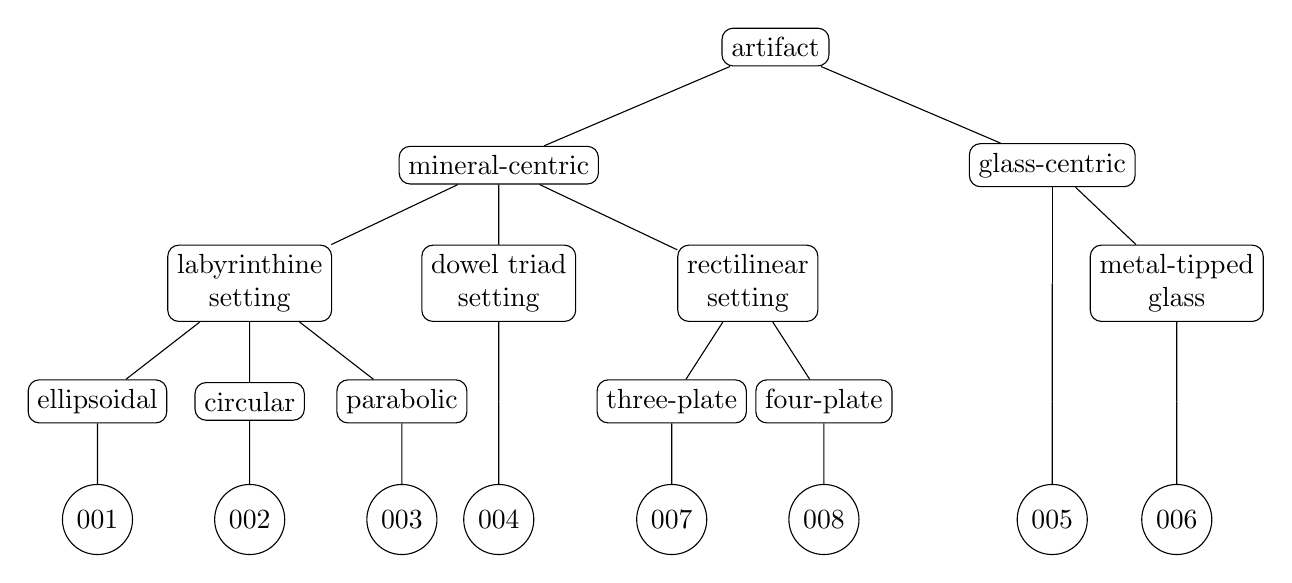
\begin{tikzpicture}[baseline,sibling distance=20em,
 every node/.style = {shape=rectangle, rounded corners, draw, align=center},
 level 2/.style = {sibling distance=9em},
 level 3/.style = {sibling distance=5.5em}]
 \node {artifact}
   child { node {mineral-centric} 
     child { node {labyrinthine\\setting} 
       child { node {ellipsoidal} 
         child { node [circle] {001} } }
       child { node {circular} 
         child { node [circle] {002} } }
       child { node {parabolic}
         child { node [circle] {003} } } }
     child { node {dowel triad\\setting} 
       child { child { node [circle] {004} } } }
     child { node {rectilinear\\setting} 
     	child { node {three-plate} 
	  child { node [circle] {007} } }
	child { node {four-plate}
	  child { node [circle] {008} } } } }
   child { node {glass-centric}
     child [sibling distance=0em] { child { child { node [circle] {005} } } }
     child { node {metal-tipped\\glass} 
       child { child { node [circle] {006} } } } };
 \end{tikzpicture}
\end{document}